\chapter{Considerações Finais}\label{chp:conclusao}

\section{Conclusão e Resultados}\label{sec:conclusao-resultados}

O combustível principal deste trabalho, fortemente compartilhado por todos os integrantes, foi a possibilidade de unir o interesse acadêmico e a incrível experiência vivenciada durante todos os anos de estudos na UFRJ com o objetivo de gerar valor para o mercado corporativo através da Visagio\cite{visagio}, empresa na qual trabalhamos há mais de três anos e formada por ex-alunos desta instituição.

Em um cliente da Visagio, onde o Redmine já era utilizado para a gestão de diversos processos na área de Suprimentos, observou-se a necessidade da implantação de fluxos de aprovação mais complexos do que o Redmine poderia oferecer por padrão. Nesse cenário, observamos uma excelente oportunidade para avaliar na prática o funcionamento da solução descrita ao longo deste trabalho.

A figura \ref{fig:process_cartao_compras} demonstra o processo para solicitação de criação de cartão de crédito corporativo. Este processo foi configurado para rodar no Activiti BPM e Redmine, através do \textit{Redmine BPM Integration Plugin} desenvolvido neste trabalho. O processo é disparado mediante a abertura de um chamado no Redmine, onde são preenchidos dados pessoais do solicitante, endereço para entrega do cartão e diretor aprovador. Após a criação do processo, o Activiti BPM imediatamente cria a próxima tarefa: \textit{Workflow Diretor}. Através do mecanismo de sincronização, uma sub-tarefa é criada no Redmine, representando a aprovação do diretor. Esta tarefa tem o responsável definido pelo preenchimento do aprovador na tarefa anterior, sendo encaminhado através do fluxo no Activiti BPM ao Redmine definindo o responsável pela tarefa. Como é possível observar no diagrama, o processo segue por mais dois níveis de aprovação, até finalmente o cartão estar aprovado para emissão e entrega ao solicitante. Caso algum dos aprovadores reprove a solicitação do cartão, o chamado é encerrado e assume o status Reprovado.

\begin{figure}[H]
\centering
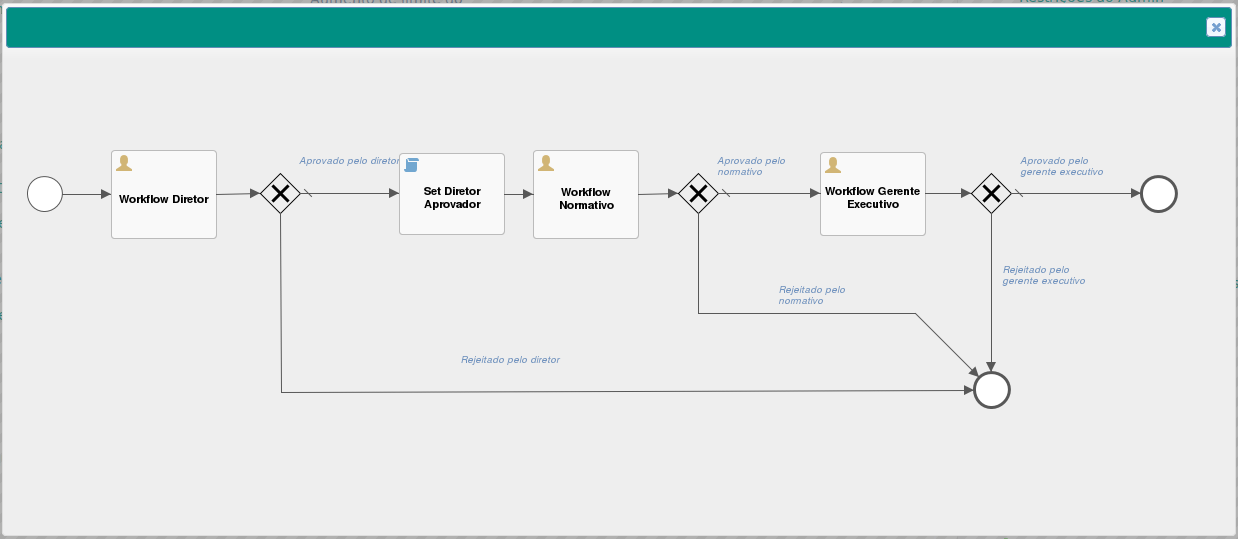
\includegraphics[width=1\textwidth]{imagens/processo_cartao_compras.png}
\caption{Modelo de processo de Criação de cartão corporativo}
\label{fig:process_cartao_compras}
\end{figure}


No caso do processo descrito, a implementação no Activiti BPM permitiu que as tarefas de aprovação fossem atribuídas automaticamente, e que a reprovação de uma etapa resultasse no encerramento do processo com o status Reprovado. Esse comportamento não seria possível de maneira simples no Redmine, diferentemente do Activiti BPM, onde a modelagem permite esse tipo de fluxo de trabalho. O processo descrito anteriormente e outros processos implantados de diferentes complexidades tiveram razão para serem implementados utilizando o plugin desenvolvido, aproveitando-se das facilidades de modelagem e fluxos proporcionados pelo BPM.

No gráfico da figura \ref{fig:grafico_processo} é possível verificar o total de criação e conclusão de três diferentes grupos de processos. Ao observarmos que todos os processos tem um alto percentual de resolução, podemos concluir que a integração entre o Redmine e o Activiti BPM funcionou conforme o esperado, e que os processos fluíram normalmente com a interação dos atores do processo através do Redmine. Além disso, não foram observados reclamações importantes referentes ao funcionamento do fluxo de trabalho. No total, foram iniciados 4.275 processos desde Março de 2016, o que representa uma média de 21 processos iniciados por dia até Setembro de 2016.

\begin{figure}[H]
\centering
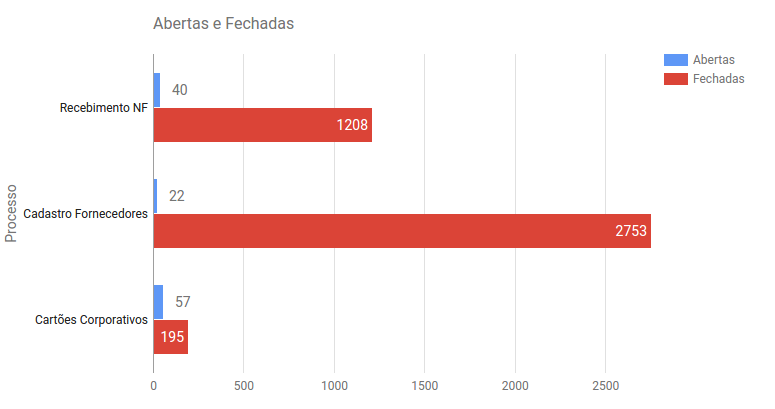
\includegraphics[width=1\textwidth]{imagens/grafico_processo.png}
\caption{Processos utilizando o plugin}
\label{fig:grafico_processo}
\end{figure}


\section{Melhorias Propostas}\label{sec:conclusao-melhorias}

Em alinhamento com a utilização de soluções de código-fonte aberto que compõem este trabalho, todo o código-fonte da integração desenvolvida está disponibilizado no GitHub da Visagio\cite{github_visagio}. O \textit{Redmine BPM Integration Plugin} segue em constante evolução através da implementação desta solução em clientes relevantes no Brasil, o que exige constantes melhorias e avanços no projeto inicial apresentado neste trabalho.

A seguir são apresentadas algumas propostas de melhorias para o seguimento deste trabalho:

\subsection{Tarefas Contínuas}

Durante a implantação, um \textit{feedback} foi recebido pelos usuários do sistema. O plugin introduziu um comportamento um pouco diferente na continuidade do processo do que era de costume no Redmine. Como explicado acima, a representação de uma tarefa humana do Activiti no Redmine é uma sub-tarefa do chamado original que representa o processo. Uma das principais razões desta mudança foi a necessidade de tratar os casos de tarefas humanas que rodam em paralelo, em que no Redmine, cada ator poderia executar sua tarefa isoladamente numa sub-tarefa. 
Esta modificação, no entanto, tirou um pouco a continuidade de um processo em que várias etapas são executadas sequencialmente por um mesmo ator, pois ele não consegue fazer isto apenas avançando as etapas numa mesma tela, mas abrindo cada vez a próxima sub-tarefa que é criada para a próxima etapa. Neste cenário, existe possibilidade de melhorias para melhorar a fluidez quando as tarefas sequenciais são executadas por um mesmo ator.

\subsection{BPMN Integrado}

Neste trabalho utilizamos o Activiti Designer para a modelagem dos processos, que é constituído basicamente do Eclipse com um plugin BPMN. Este cenário apresenta-se pouco prático para usuários sem conhecimento de TI. Nesse sentido, observamos a oportunidade de prover uma modelagem de processos fácil e integrada ao Redmine. Assim, o usuário poderia criar seu processo diretamente na ferramenta, com uma interface simples e online, sem a necessidade de contato com aplicações específicas de desenvolvimento.

Já existem iniciativas similares neste sentido, como o Activiti Modeler\cite{activiti_modeler}, exibido na figura \ref{fig:activiti_modeler}. Portanto, uma melhoria interessante seria acoplar esta ferramenta ao Redmine e avaliar as melhorias necessárias para deixar sua utilização agradável e simples numa única ferramenta.

\begin{figure}[H]
\centering
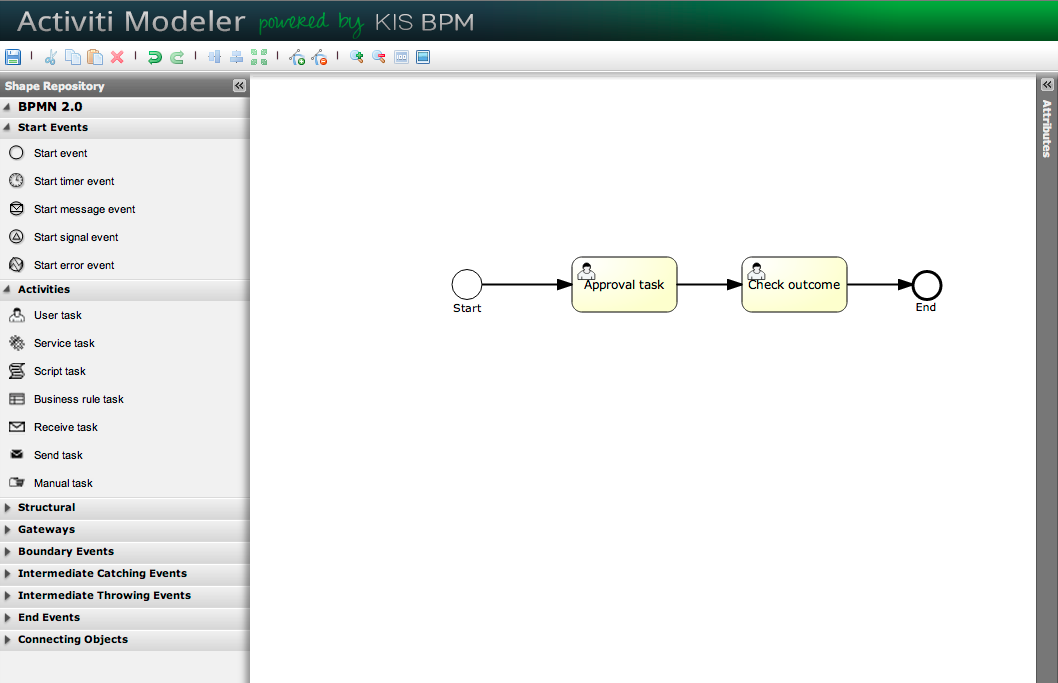
\includegraphics[width=1\textwidth]{imagens/activiti_modeler.png}
\caption{Activiti Modeler}
\label{fig:activiti_modeler}
\end{figure}

\subsection{BRM Integrado}

Uma característica bastante comum em sistemas BPMS é a presença de um BRM (\textit{Business Rules Management}) para gestão de regras de negócio nos processos. O Activiti BPM suporta a integração com o Drools, uma aplicação \textit{web} desenvolvida em Java especialista em BRM. A figura \ref{fig:drools} apresenta uma tabela de decisão no Drools, que pode ser configurada pelo usuário para definir uma regra de negócio baseada em intervalo de valores estabelecendo, por exemplo, a alçada de aprovação em um processo de pagamento.

\begin{figure}[H]
\centering
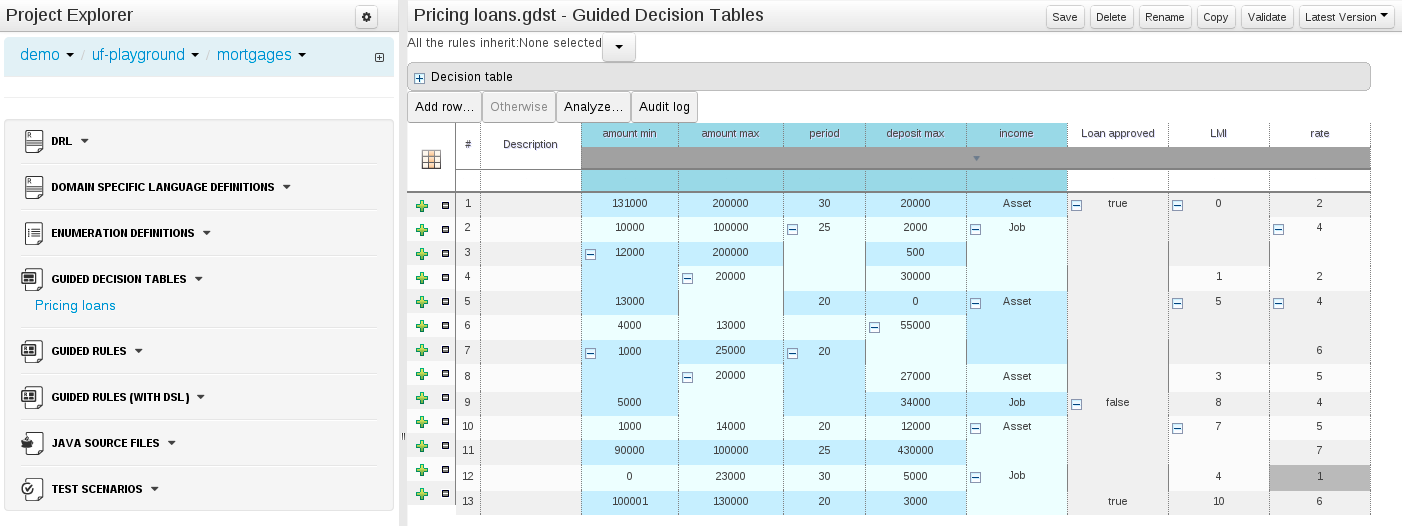
\includegraphics[width=1\textwidth]{imagens/drools_decision_table.png}
\caption{Tabela de decisão no Drools}
\label{fig:drools}
\end{figure}

Uma proposta de evolução no contexto da integração do BPMS com o Redmine, seria o desenvolvimento de plugin BRM, de forma a facilitar a gestão de regras de negócio para processos BPM diretamente no Redmine.

\subsection{BPMS Genérico}

Conforme tentativa apresenta na seção \ref{sec:cenario-integracao-genérica}, esta melhoria proporcionaria uma cadama genérica de integração de qualquer BPMS ao Redmine, flexibilizando assim a escolha do BPMS ou até mesmo a integração com um BPMS que já esteja em uso pela empresa. 